\section{Superfície equipotencial e energia elétrica}

\frame{
	\frametitle{Superfície equipotencial}
	\begin{block}{Definição}
		Chamamos uma superfície de equipotencial quando, numa região de campo elétrico, \textbf{todos os seus pontos apresentam o mesmo potencial elétrico}. Uma superfície equipotencial pode apresentar diversas formas geométricas.
	\end{block}
}

\frame{
	\frametitle{Superfície equipotencial}
	\begin{block}{Revisão}
		Vimos que o valor do potencial num ponto $P$ depende do valor da carga elétrica geradora $Q$, da distância $d$ entre a carga e o ponto $P$ e do meio onde está inserida. \\
		$$V = K \ \dfrac{Q}{d}$$
		\begin{itemize}
			\item Quando $A$ e $B$ estão na mesma superfície equipotencial, então $V_A = V_B$, apresentando, portanto, uma variação de potencial elétrica nula, igual à zero.
		\end{itemize}
	\end{block}
}

\frame{
	\frametitle{Superfícies equipotenciais criadas por uma carga pontual}
	\begin{block}{Superfícies esféricas concêntricas}
		Quando uma carga puntiforme cria um campo elétrico, as superfícies equipotenciais desse campo são esféricas com centro na carga.
	\end{block}

	\setmyunit{0.5cm}

	\begin{minipage}{0.49\linewidth}
		\centering
		
		\begin{tikzpicture}
			\foreach \x in {0,45,...,330}
				\draw[red,-Latex] (0,0) -- (\x:4);
			
			\foreach \y in {0,1,2} {
				\foreach \x in {45,135} {
					\draw (0,0) ++(\x:\y.85) -- ++(-\x:0.15) -- ++(\x:0.15) ++(\x:-0.15) ++(0,0.075) node {$ \cdot $};
				}
			
				\foreach \x in {-45,-135} {
					\draw (0,0) ++(\x:\y.85) -- ++(-\x:0.15) -- ++(\x:0.15) ++(\x:-0.15) ++(0,-0.125) node {$ \cdot $};
				}
			
				\draw (0,0) ++(\y.85,0) -- ++(0,0.15) -- ++(0.15,0) -- ++(-0.075,-0.1) node {$ \cdot $};
			
				\draw (0,0) ++(90:\y.85) -- ++(0.15,0) -- ++(0,0.15) ++(-0.075,-0.1) node {$ \cdot $};
			
				\draw (0,0) ++(270:\y.85) -- ++(-0.15,0) -- ++(0,-0.15) ++(0.075,0.075) node {$ \cdot $};
				
				\draw (0,0) ++(-\y.85,0) -- ++(0,0.15) -- ++(-0.15,0) -- ++(0.075,-0.1) node {$ \cdot $};
			}
			
			\draw[blue] (0,0) circle (1) circle (2) circle (3);
			
			\fill (0,0) circle (2pt) node[below,xshift=2.5pt,yshift=-1pt] {$ q $};
			
			\fill (1,0) circle (1pt) node[below,xshift=2pt] {$ A $} (2,0) circle (1pt) node[below,xshift=2pt] {$ B $} (3,0) circle (1pt) node[below,xshift=3pt] {$ C $};
		\end{tikzpicture}
		
		Carga puntiforme positiva
		\[ V_A > V_B > V_C \]
	\end{minipage}
	\hfill
	\begin{minipage}{0.49\linewidth}
		\centering
		
		\begin{tikzpicture}
		\foreach \x in {0,45,...,330} {
			\draw[red] (0,0) -- (\x:4);
			\draw[red, -Latex] (\x:4) -- +(\x:-0.5);
		}
		
		\foreach \y in {0,1,2} {
			\foreach \x in {45,135} {
				\draw (0,0) ++(\x:\y.85) -- ++(-\x:0.15) -- ++(\x:0.15) ++(\x:-0.15) ++(0,0.075) node {$ \cdot $};
			}
			
			\foreach \x in {-45,-135} {
				\draw (0,0) ++(\x:\y.85) -- ++(-\x:0.15) -- ++(\x:0.15) ++(\x:-0.15) ++(0,-0.125) node {$ \cdot $};
			}
			
			\draw (0,0) ++(\y.85,0) -- ++(0,0.15) -- ++(0.15,0) -- ++(-0.075,-0.1) node {$ \cdot $};
			
			\draw (0,0) ++(90:\y.85) -- ++(0.15,0) -- ++(0,0.15) ++(-0.075,-0.1) node {$ \cdot $};
			
			\draw (0,0) ++(270:\y.85) -- ++(-0.15,0) -- ++(0,-0.15) ++(0.075,0.075) node {$ \cdot $};
			
			\draw (0,0) ++(-\y.85,0) -- ++(0,0.15) -- ++(-0.15,0) -- ++(0.075,-0.1) node {$ \cdot $};
		}
		
		\draw[blue] (0,0) circle (1) circle (2) circle (3);
		
		\fill (0,0) circle (2pt) node[below,xshift=2.5pt,yshift=-1pt] {$ q $};
		
		\fill (1,0) circle (1pt) node[below,xshift=2pt] {$ A $} (2,0) circle (1pt) node[below,xshift=2pt] {$ B $} (3,0) circle (1pt) node[below,xshift=3pt] {$ C $};
		\end{tikzpicture}
		
		Carga puntiforme negativa
		\[ V_A < V_B < V_C \]
	\end{minipage}
	

%	\centerline{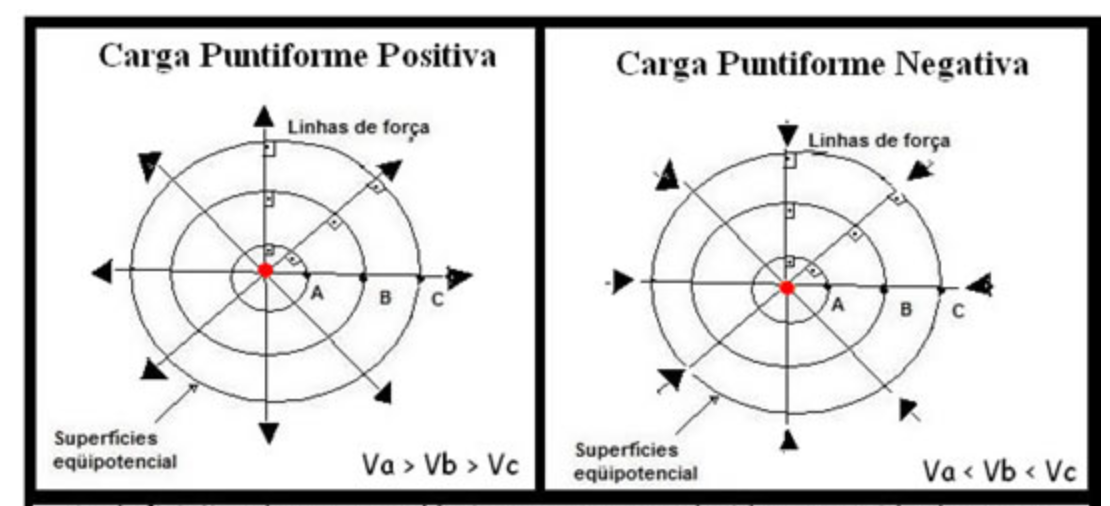
\includegraphics[width=0.9\linewidth]{Figuras/Ch10/equipotencial1.PNG}}
}

\frame{
	\frametitle{Superfície equipotencial}
	\begin{block}{Propriedade $\#$01}
		O \textbf{trabalho} da força elétrica durante o deslocamento de uma carga elétrica puntiforme sobre uma superfície equipotencial é \textbf{nulo}.
	\end{block}

	\begin{block}{Propriedade $\#$02}
		Uma superfície equipotencial é sempre interceptada \textbf{perpendicularmente} ($\ang{90}$) pelas linhas de força de um campo elétrico, e, consequentemente, ortogonais ao vetor campo elétrico $\vec{E}$. Dessa maneira, conhecendo-se as linhas de força de um campo elétrico, fica mais fácil representar as superfícies equipotenciais.
	\end{block}
}

\frame{
	\frametitle{Energia potencial elétrica}
	\begin{block}{Introdução}
		Vamos considerar uma carga elétrica pontual $q$ que se encontra no campo elétrico de uma carga geradora $Q$. Se essa carga se move de um ponto $P$ deste campo elétrico até um ponto infinitamente distante, o trabalho da força elétrica é dado por:
		$$\tau_{P\infty} = q(V_p - V_\infty) = q \cdot V_p$$
	\end{block}
}

\frame{
	\frametitle{Energia potencial elétrica}
	\begin{block}{Definição}
		Ao trabalho realizado para deslocar uma carga elétrica $q$ de um ponto $P$ de um campo até o infinito, damos o nome de \textbf{energia potencial elétrica}.
		$$\boxed{E_p(P) = \tau_{P\infty} = q \cdot V_p}$$
	\end{block}
}

\frame{
	\frametitle{Energia potencial elétrica}
	\begin{block}{Trabalho}
		Lembrando que
		$$\tau_{AB} = q(V_A - V_B)$$
		\begin{itemize}
			\item Nos pontos $A$ e $B$ a carga $q$ tem energias potenciais dadas por:
			      \begin{itemize}
				      \item $E_p(A) = q \cdot V_A$
				      \item $E_p(B) = q \cdot V_B$
			      \end{itemize}
		\end{itemize}
	\end{block}
}

\frame{
	\frametitle{Energia potencial elétrica}
	\begin{block}{Trabalho}
		Logo, $\tau_{AB} = E_p(A) - E_p(B)$, isto é, o trabalho da força elétrica mede a diferença entre as energias potenciais inicial e final da carga $q$. No deslocamento espontâneo, como $\tau$ é sempre positivo, \textbf{uma carga sofre sempre uma diminuição de sua energia potencial}.
	\end{block}
}

\frame{
	\frametitle{Energia potencial elétrica}
	\begin{block}{Observações}
		\begin{itemize}
			\item O campo elétrico é um \textbf{campo conservativo} e nele, como acontece no campo gravitacional, \textbf{o trabalho não depende da trajetória da carga} entre a posição final e inicial.
			\item As cargas $Q$ e $q$ devem ser consideradas com seu \textbf{valor algébrico}, e não em módulo.
		\end{itemize}
	\end{block}
}

\frame{
	\frametitle{Elétron-Volt}
	\begin{block}{Definição}
		Definimos o elétron-volt (\si{\electronvolt}) como sendo o trabalho realizado pela força elétrica que age sobre um \textbf{elétron} quando esse se desloca espontaneamente entre dois pontos de um campo elétrico onde há uma d.d.p. de \textbf{1 Volt}.
		$$\boxed{\SI{1}{\electronvolt} = \SI{1.6e-19}{\joule}}$$
	\end{block}
}

\section*{Exercícios}

\frame{
	\frametitle{Exercícios}
	\begin{block}{}

		01. (PUC-SP) Um elétron-volt (\si{\electronvolt}) é, por definição, a energia cinética adquirida por um
		elétron quando acelerado, a partir do repouso, por uma diferença de potencial de \SI{1.0}{\volt}.
		Considerando a massa do elétron \SI{9.0e-31}{\kilogram} e sua carga elétrica em valor absoluto \SI{1.6e-19}{\coulomb}, encontre a velocidade do elétron com energia cinética \SI{1.0}{\electronvolt}.

		\vspace{0.5cm}

		02. Considere as superfícies equipotenciais a seguir, $S_1$, $S_2$ e $S_3$, com seus respectivos potenciais elétricos indicados, e determine o trabalho realizado pela força elétrica que atua em uma partícula de carga elétrica \SI{2}{\milli\coulomb} , quando essa partícula se desloca do ponto $A$ ao ponto $D$.
	\end{block}
	\centerline{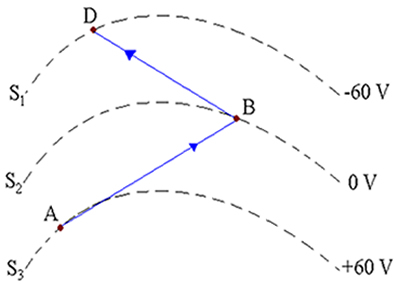
\includegraphics[width=0.3\linewidth]{Figuras/Ch10/exercicio.jpg}}
}


\section*{Referências}

\frame{
	\frametitle{Referências e Exercícios Complementares}
	\begin{itemize}
		\item Física, Ciência e Tecnologia – Vol 3. PENTEADO, Paulo César M; TORRES, Carlos Magno A. Ed. Moderna (2006)
	\end{itemize}
	%\centering{\alert{Página 36 - \textbf{1.6.1 até 1.6.5, 1.6.17 até 1.6.19}}} \\
	%https://www.youtube.com/watch?v=IUgS7Uw-qBI
	\centering{\alert{Lista de exercícios 10}}
}